The first attempt to generate artificial scans was based on the variant autoencoder architecture proposed in \cite{rombach2022high}. The implementation was based on the Monai\cite{Cardoso_MONAI_An_open-source_2022} example available on Github\footnote{\url{https://github.com/Project-MONAI/GenerativeModels/blob/e7cc989cdce440a7bff1cce22fff1caf760f39cd/tutorials/generative/3d_autoencoderkl/3d_autoencoderkl_tutorial.ipynb}} and adjusted to Pytorch Lightning.
\paragraph{Model configuration}

\begin{figure}[H]
\minipage{0.49\textwidth}
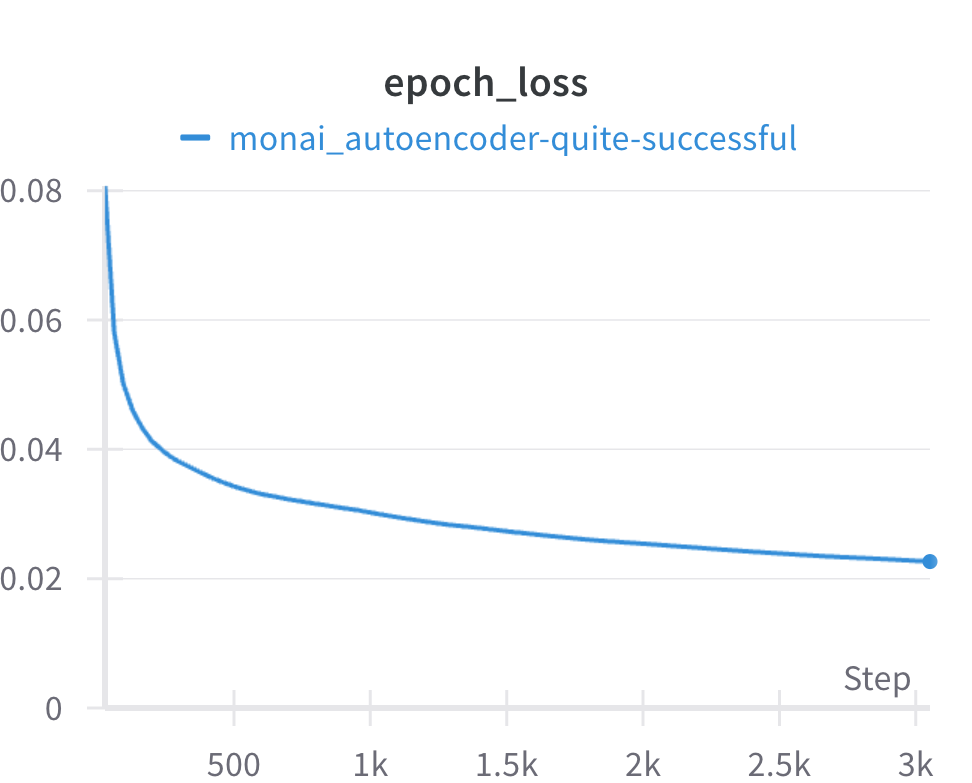
\includegraphics[width=\linewidth]{detailed_engineering/Monai Autoencoder/charts/epoch_loss.png}
\caption{}
\endminipage\hfill
\minipage{0.49\textwidth}
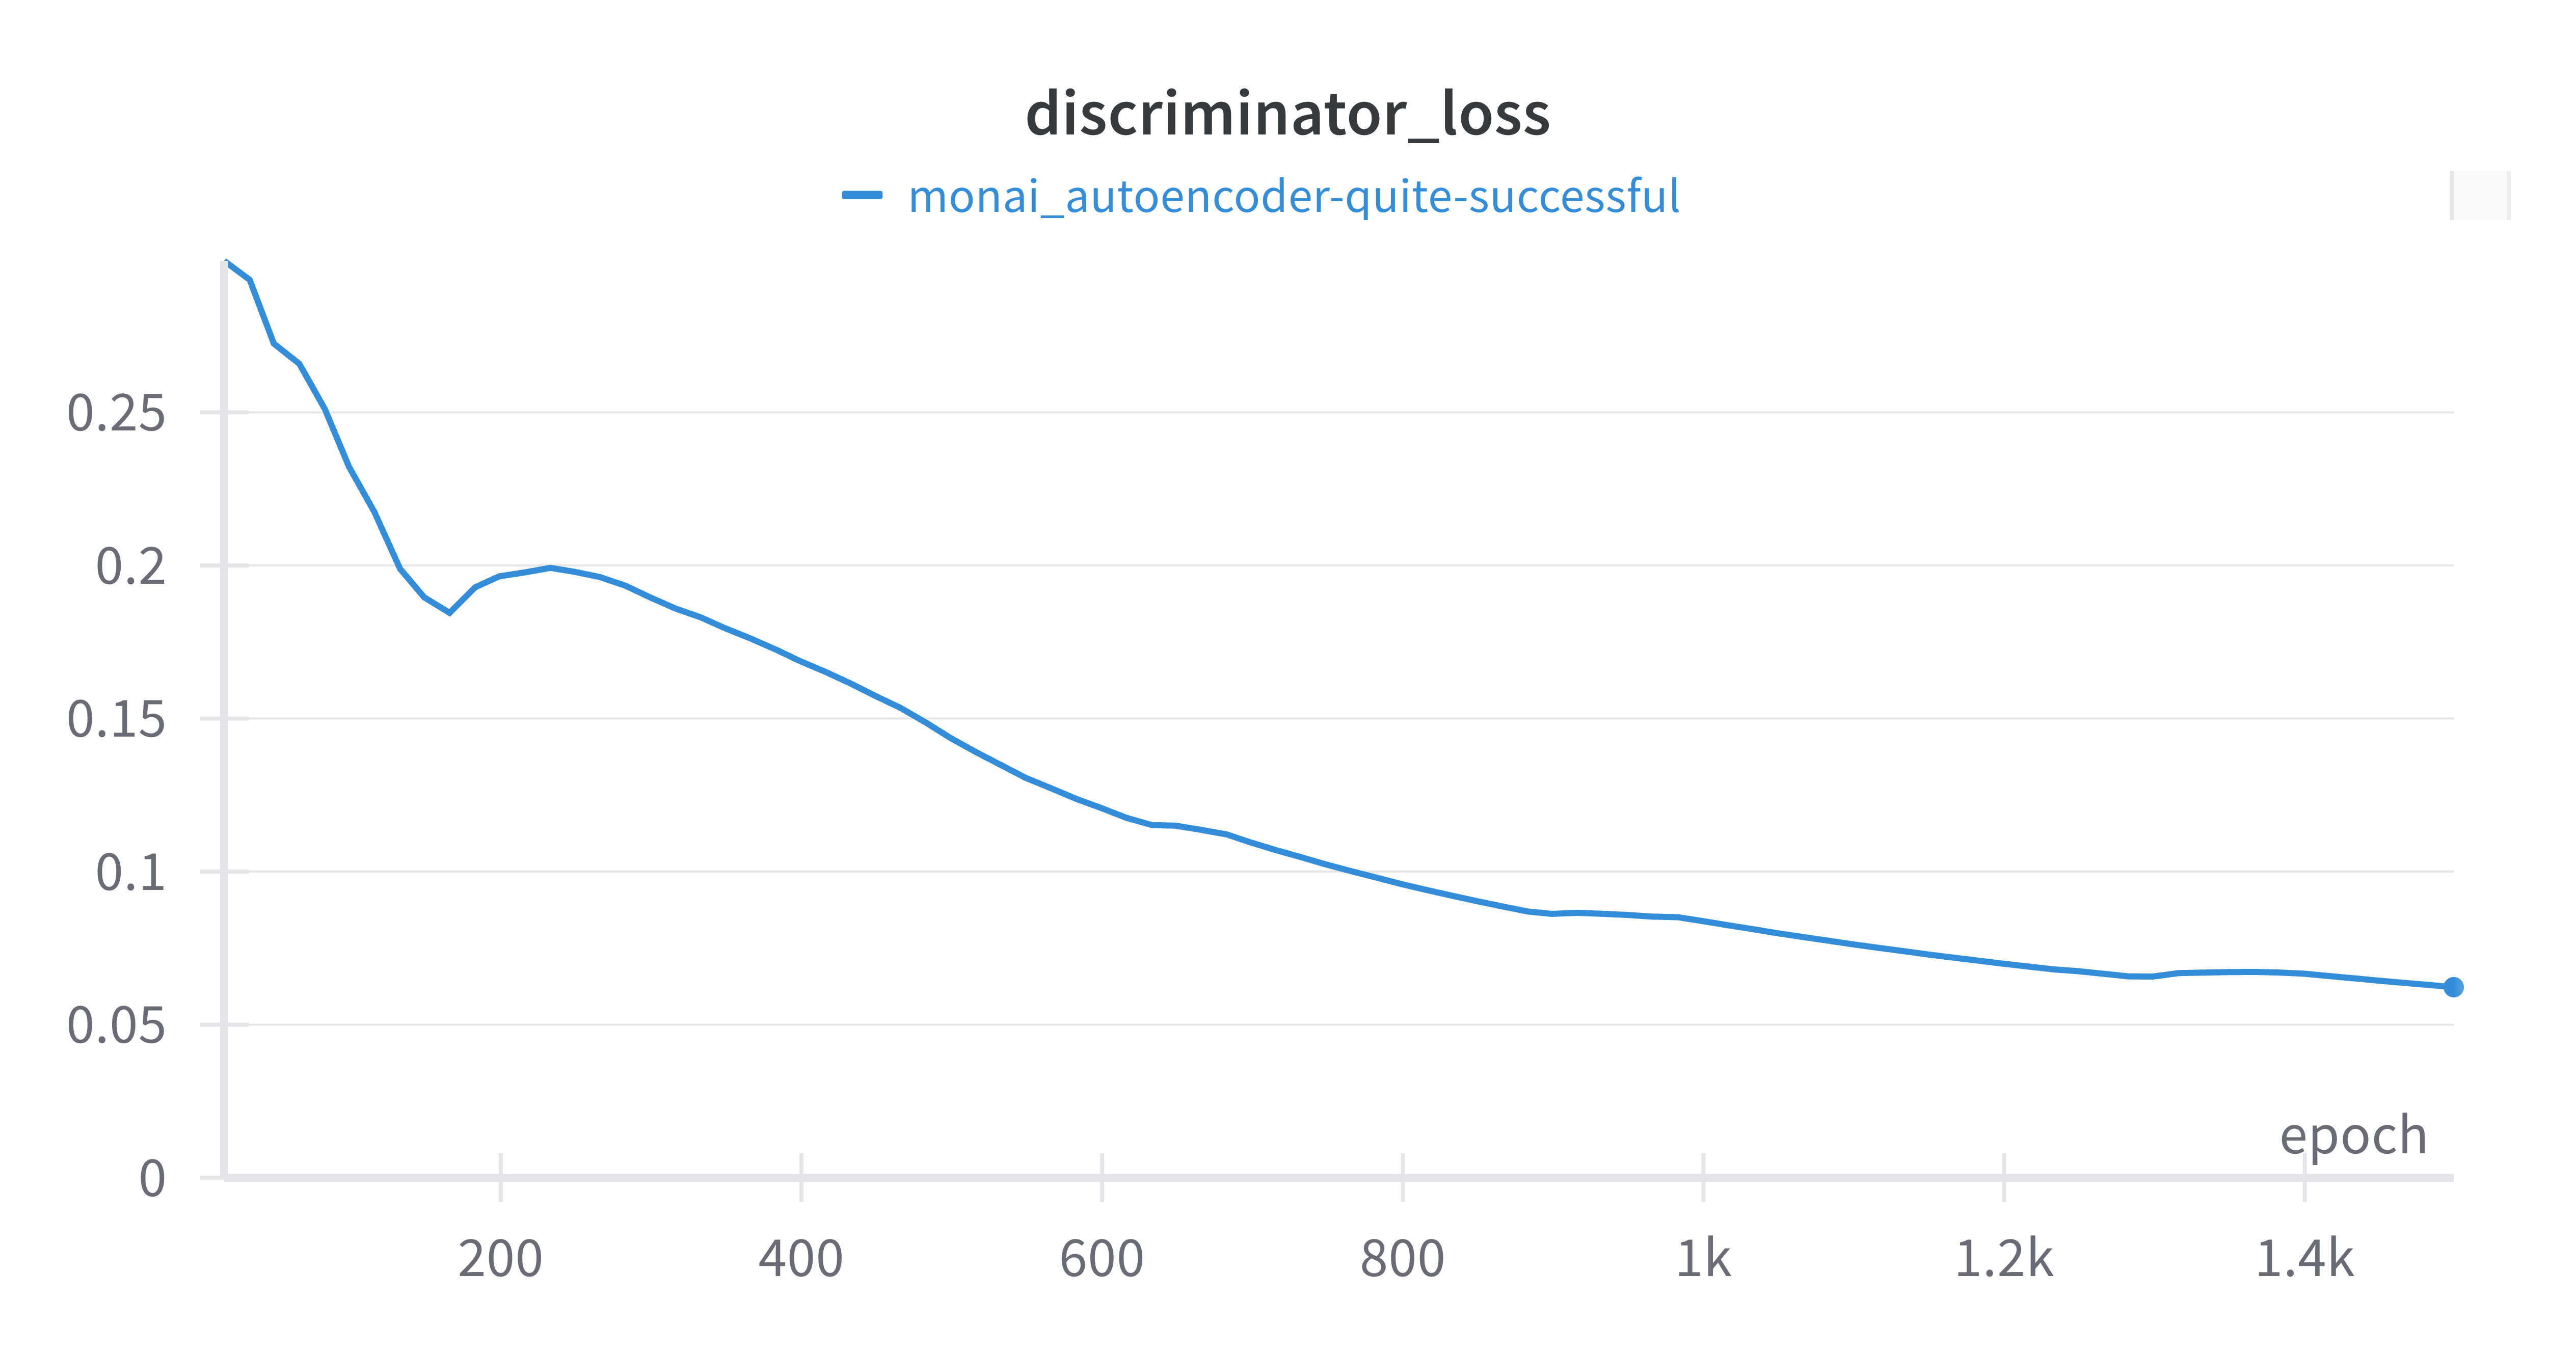
\includegraphics[width=\linewidth]{detailed_engineering/Monai Autoencoder/charts/discriminator_loss.png}
\caption{}
\endminipage
\end{figure}

\begin{figure}[H]
\minipage{0.49\textwidth}
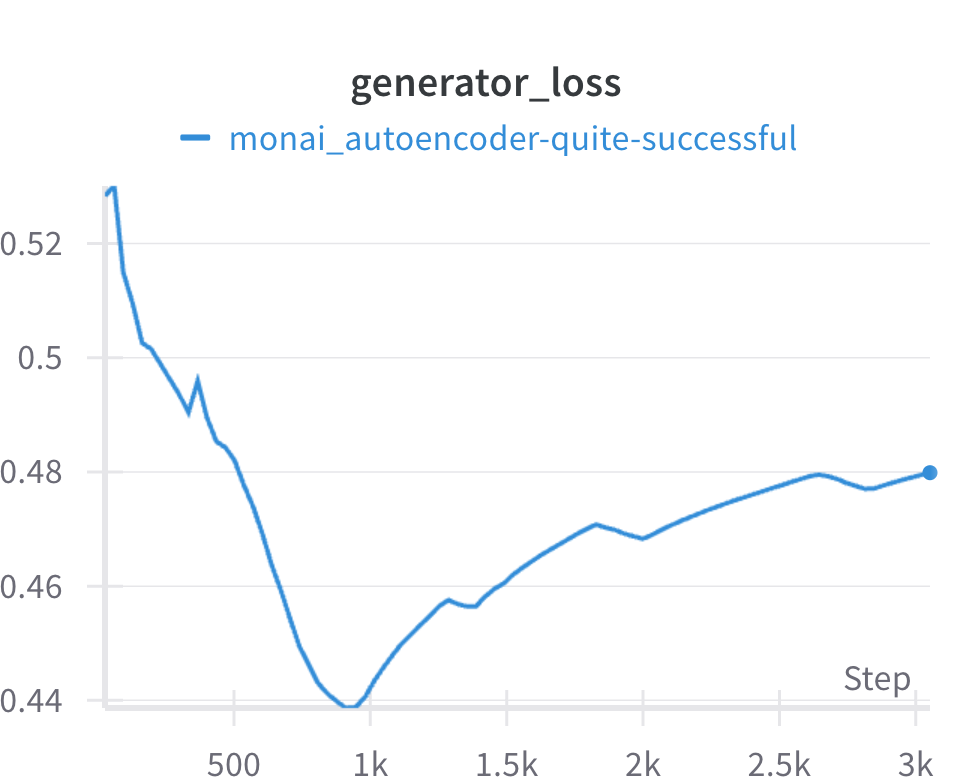
\includegraphics[width=\linewidth]{detailed_engineering/Monai Autoencoder/charts/generator_loss.png}
\caption{}
\endminipage\hfill
\minipage{0.49\textwidth}
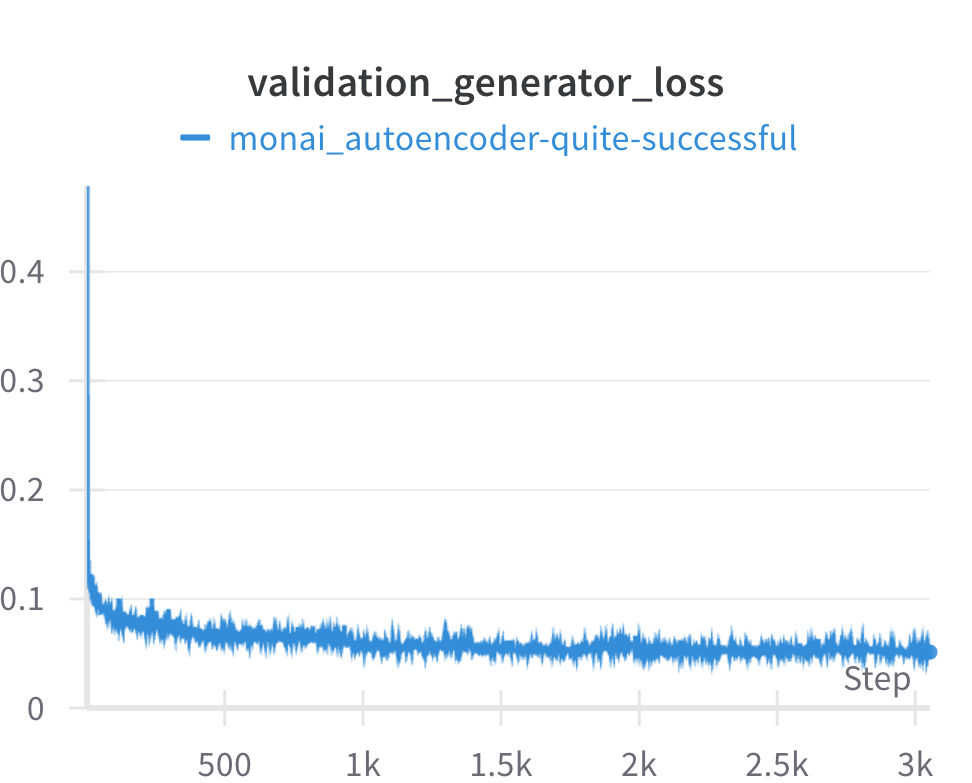
\includegraphics[width=\linewidth]{detailed_engineering/Monai Autoencoder/charts/val_generator_loss.png}
\caption{}
\endminipage
\end{figure}


\begin{figure}[H]
% \minipage{0.49\textwidth}
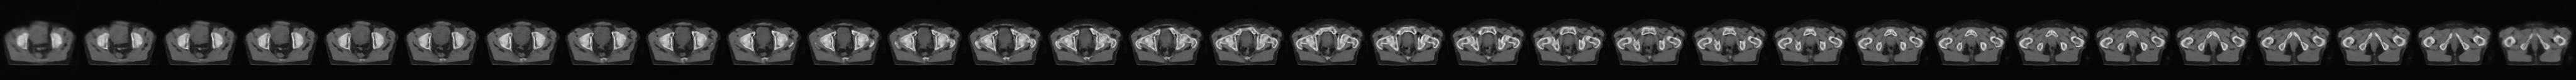
\includegraphics[width=\linewidth]{detailed_engineering/Monai Autoencoder/charts/reconstruction.png}
\caption{}
% \endminipage\hfill
% \minipage{0.49\textwidth}
% \includegraphics[width=\linewidth]{charts/Section-4-Panel-5-z2xepgyu7}
% \caption{}
% \endminipage
\end{figure}
d




\paragraph{LDM Attempt 1}\mbox{}\\

In this attempt $z$ was sampled from $\mathcal{N}(0,1)$ and passed through the decoder. 

\begin{figure}[H]
\minipage{0.49\textwidth}
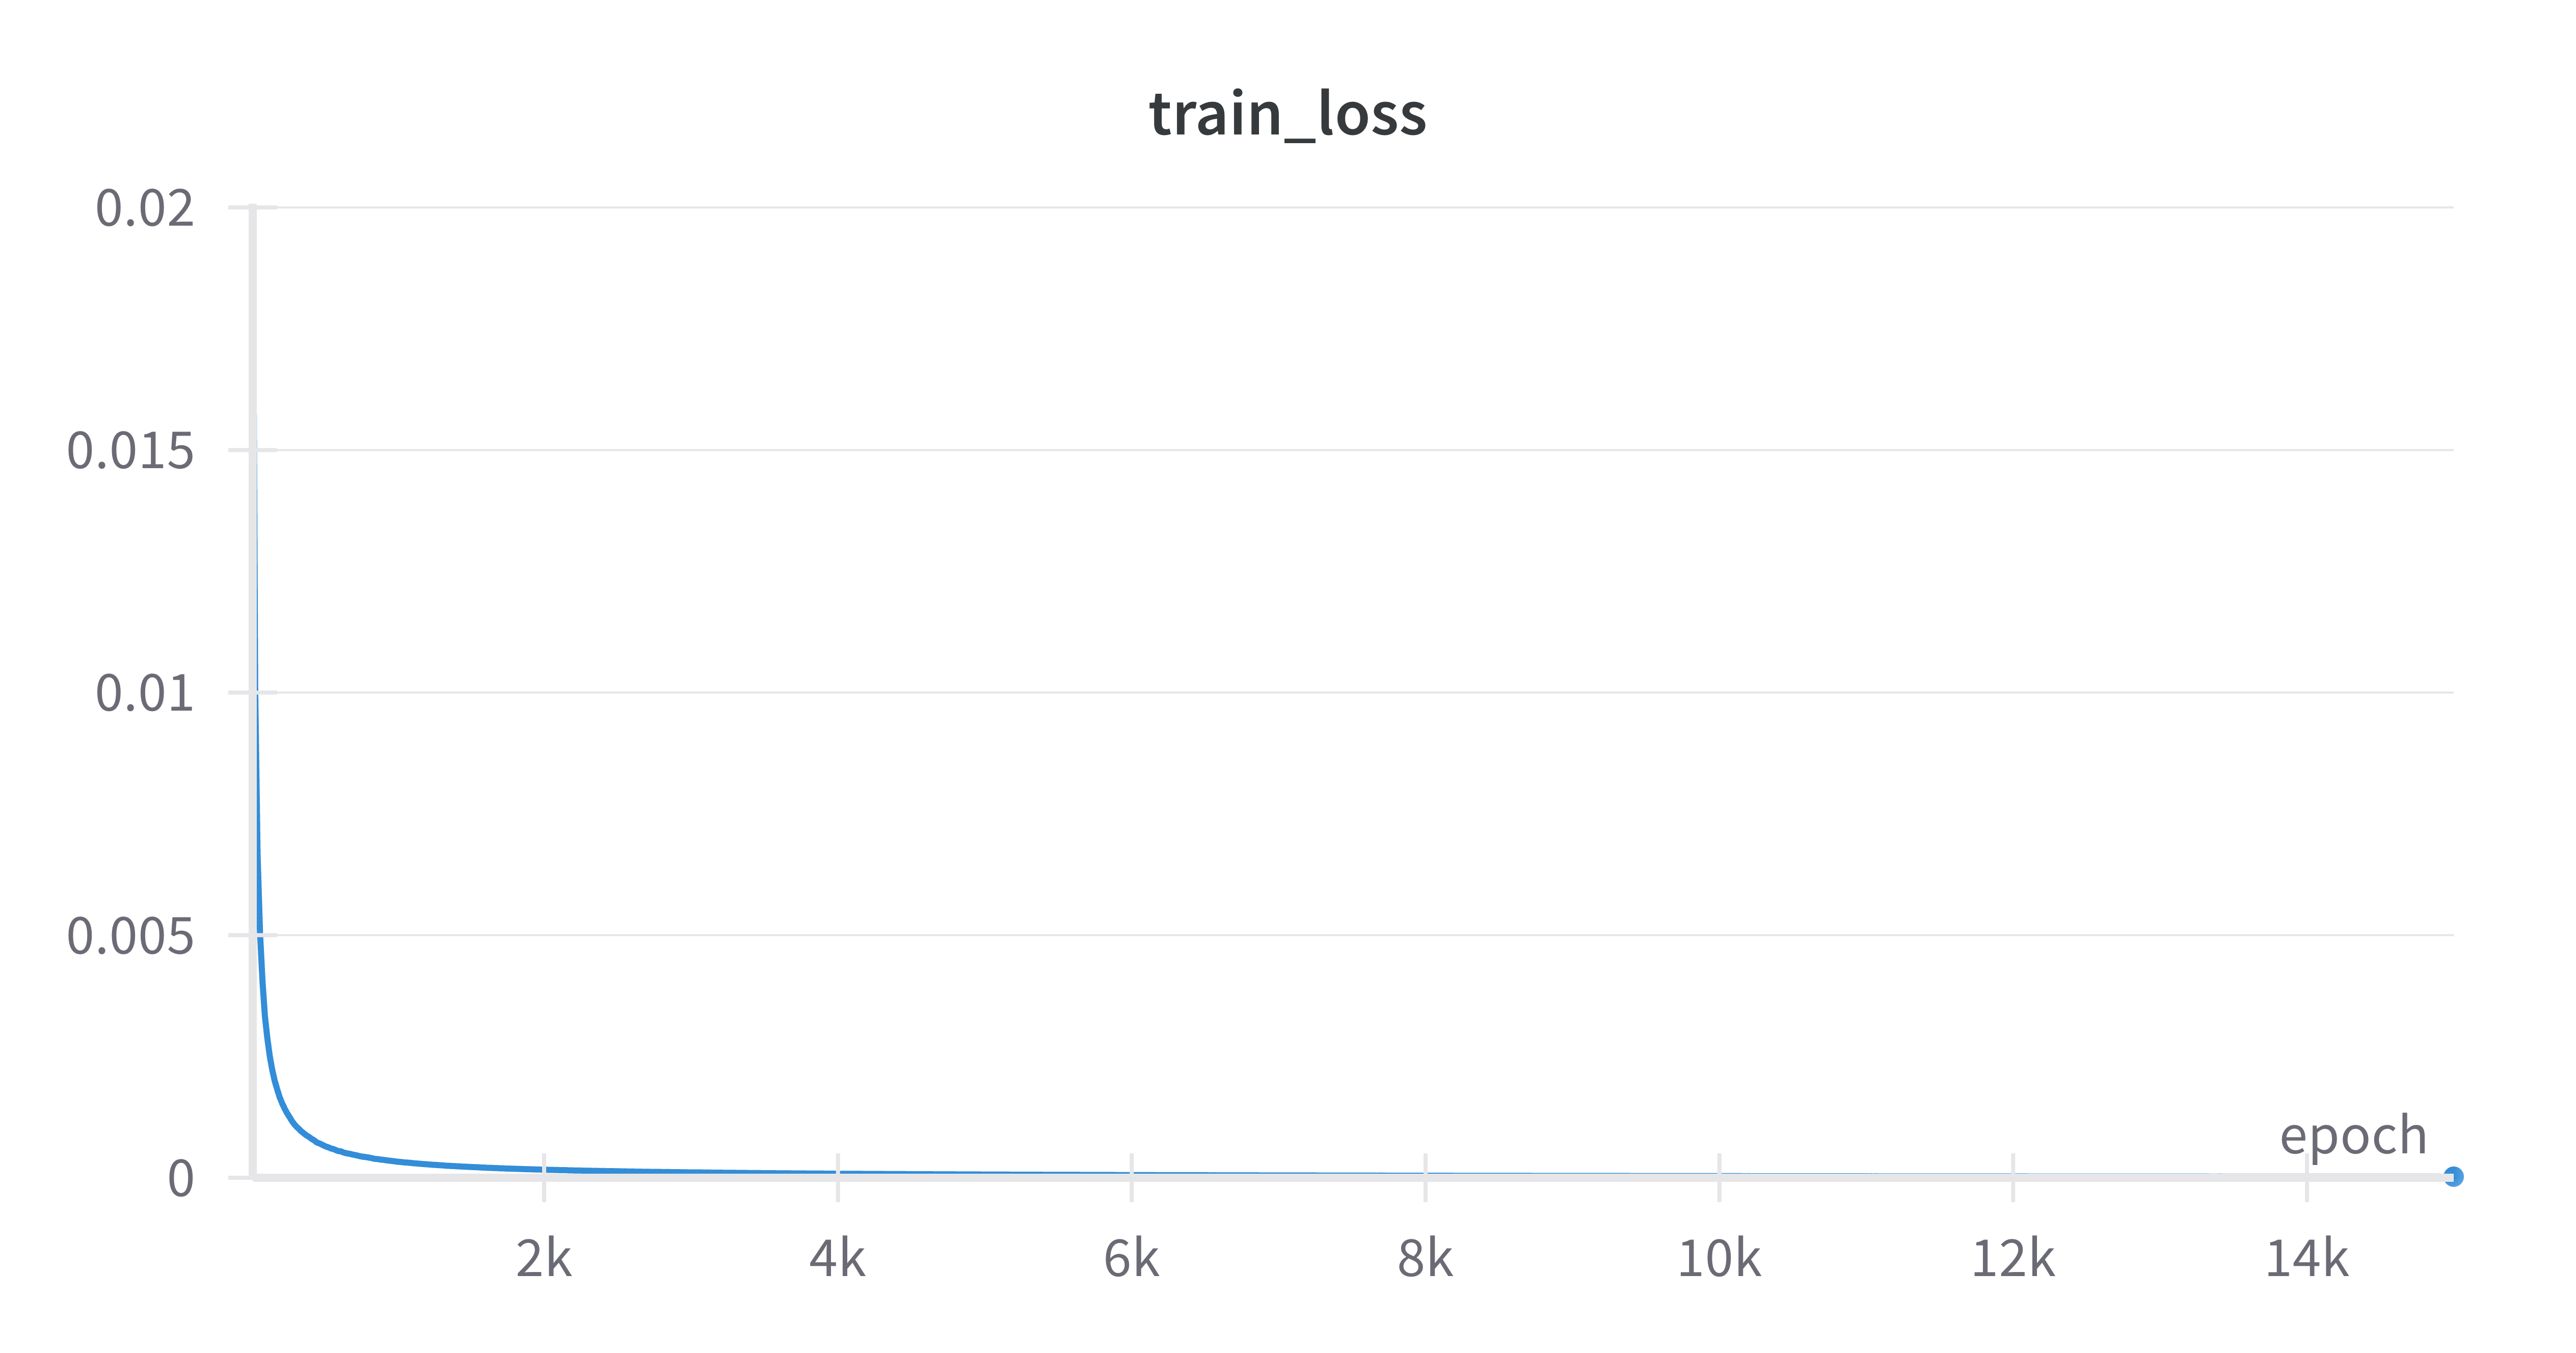
\includegraphics[width=\linewidth]{detailed_engineering/Monai Diffusion - Attempt 1/charts/train_loss.png}
\caption{}
\endminipage\hfill
\minipage{0.49\textwidth}
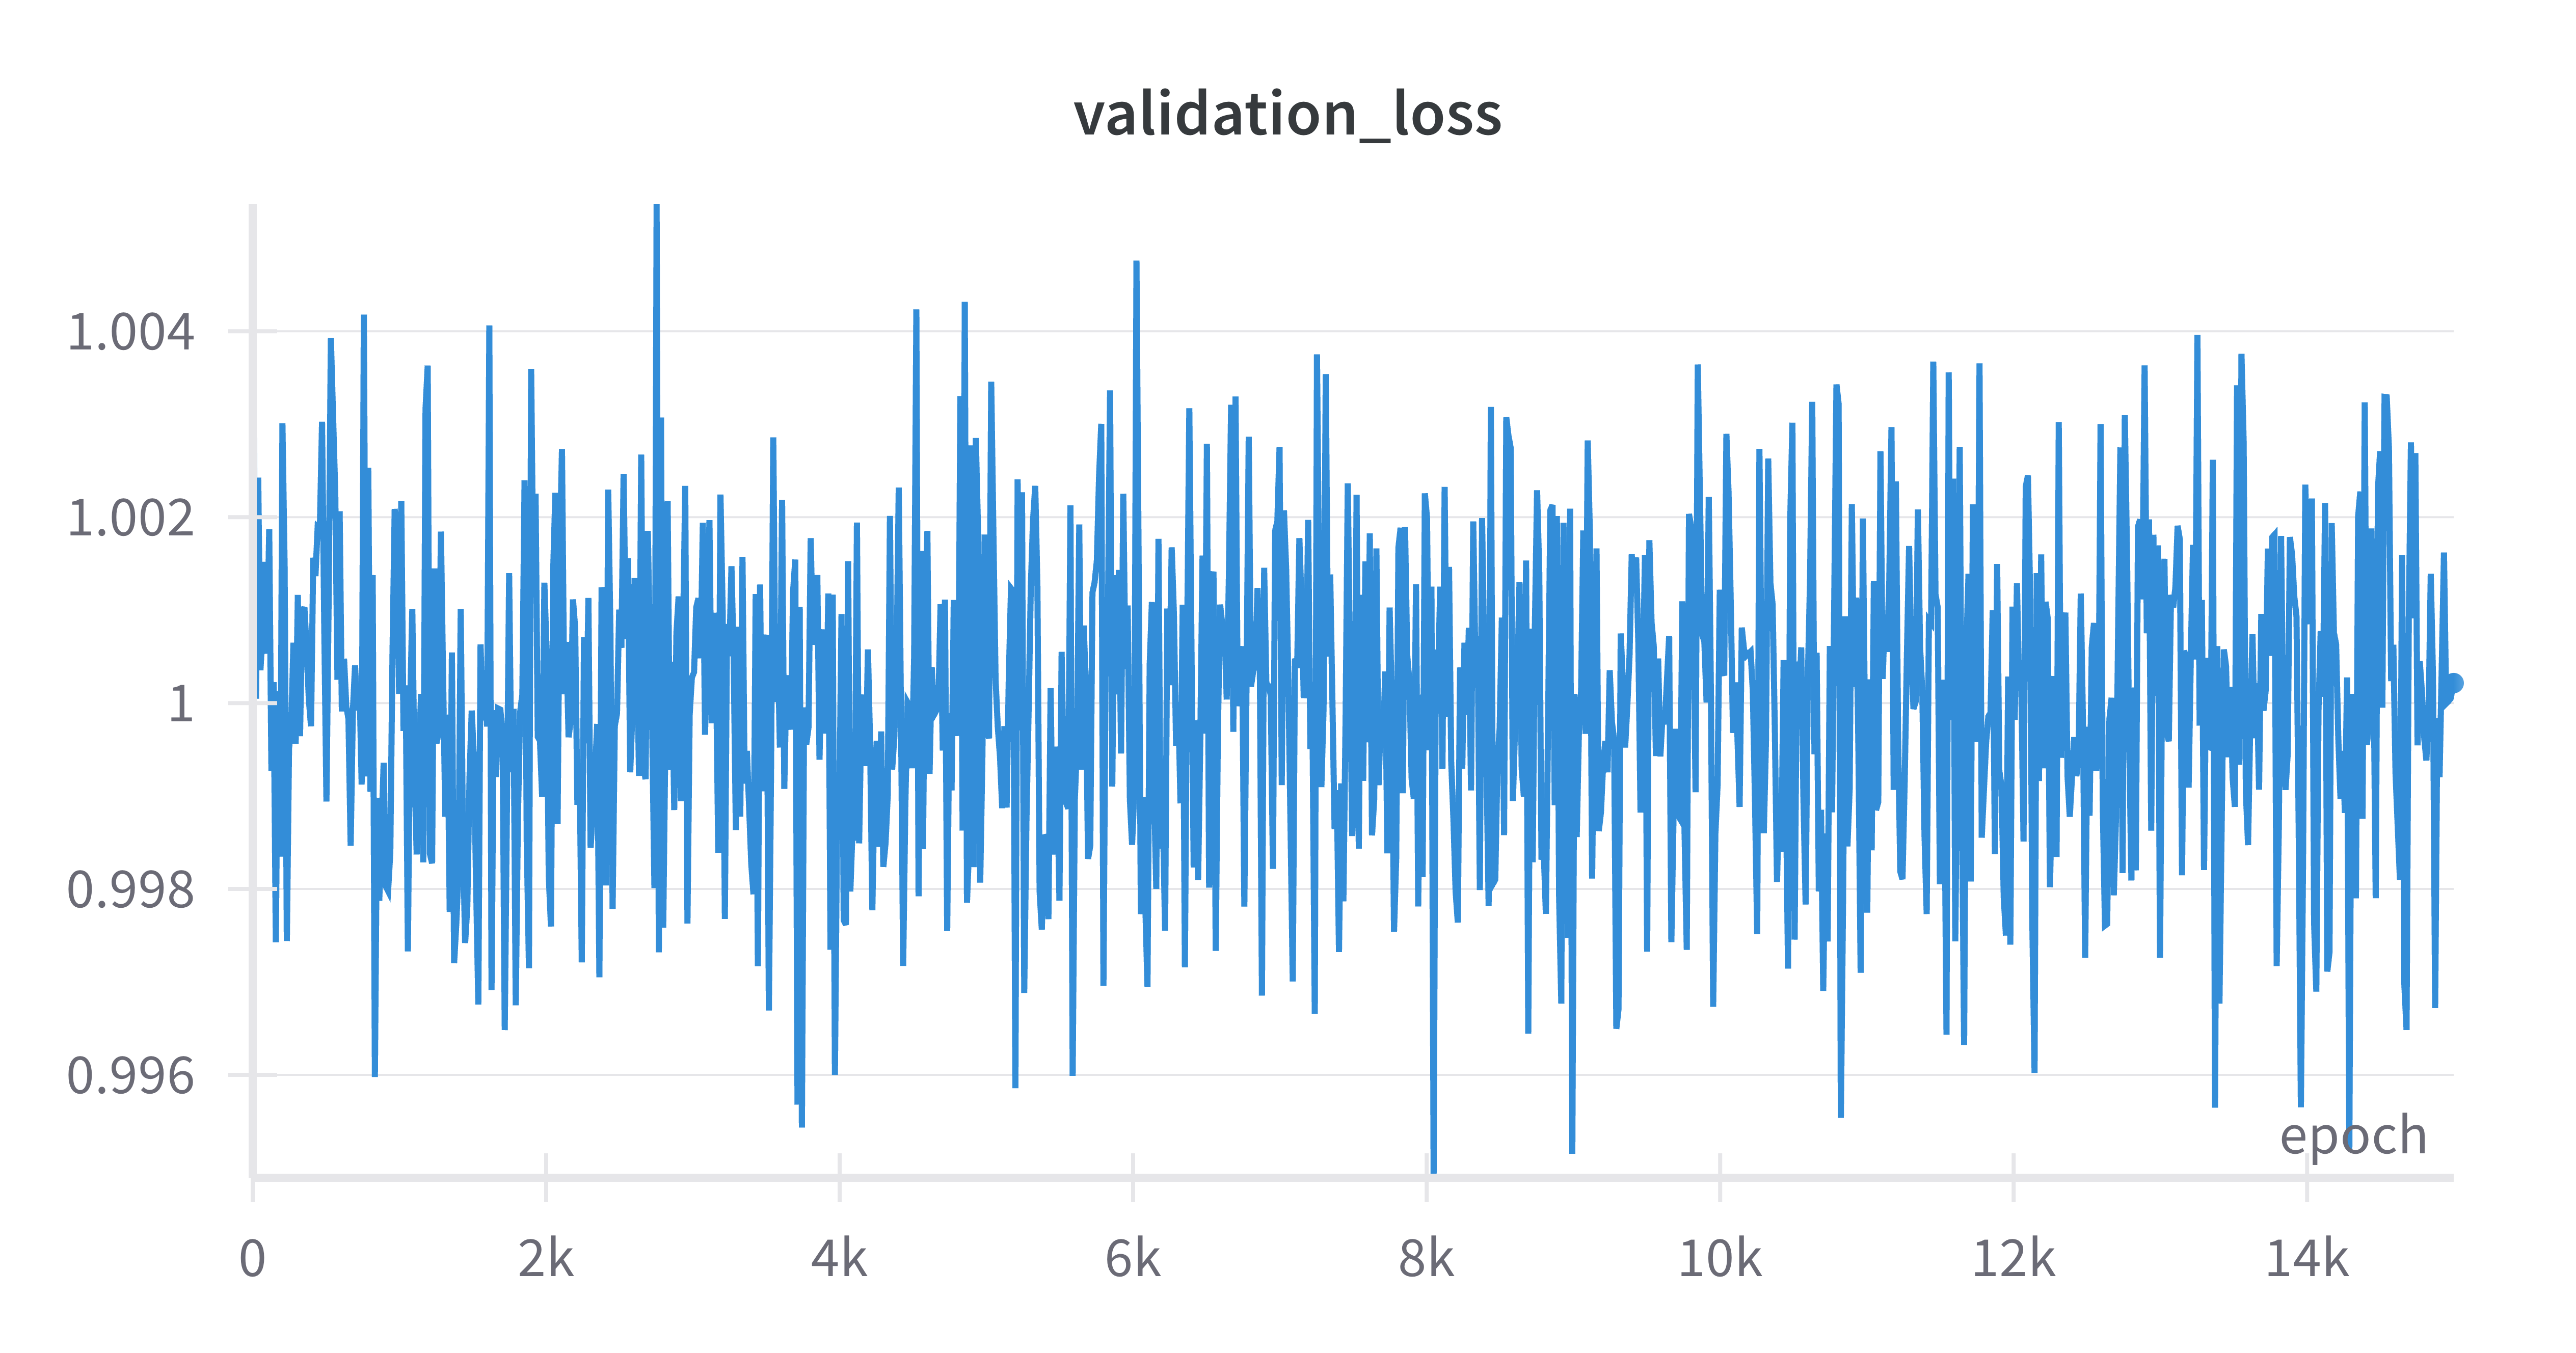
\includegraphics[width=\linewidth]{detailed_engineering/Monai Diffusion - Attempt 1/charts/validation_loss.png}
\caption{}
\label{fig:ldm_a1_val_loss}
\endminipage
\end{figure}


\begin{figure}[H]
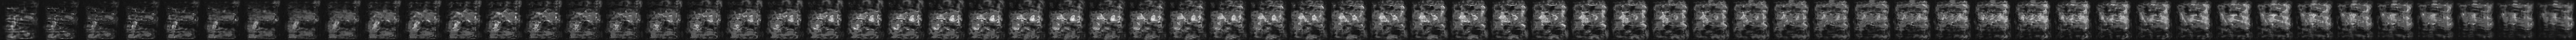
\includegraphics[width=\linewidth]{detailed_engineering/Monai Diffusion - Attempt 1/charts/generation.png}
\caption{Unsuccessful generation of synthetic CT scan.}
\label{fig:attempt1-generation}
\end{figure}

Generation was unsuccessful\ref{fig:attempt1-generation}. The validation loss did not decrease\ref{fig:ldm_a1_val_loss}.


\paragraph{LDM Attempt 2}\mbox{}\\

\indent In this attempt instead of creating noise from $\sim\mathcal{N}(0,1)$, the noise was generated from $N(\mu, \sigma)$ where $\mu$ is the mean of the training data $z_{\mu}$ and $\sigma$ is the mean of $z_{\sigma}$ obtained from the training data set (25 samples).

\paragraph{Model configuration}\mbox{}\\
The configuration was the same as in Attempt 1. The only difference was in the noise generation approach.

\paragraph{Training}\mbox{}\\
\begin{figure}[H]
\minipage{0.49\textwidth}
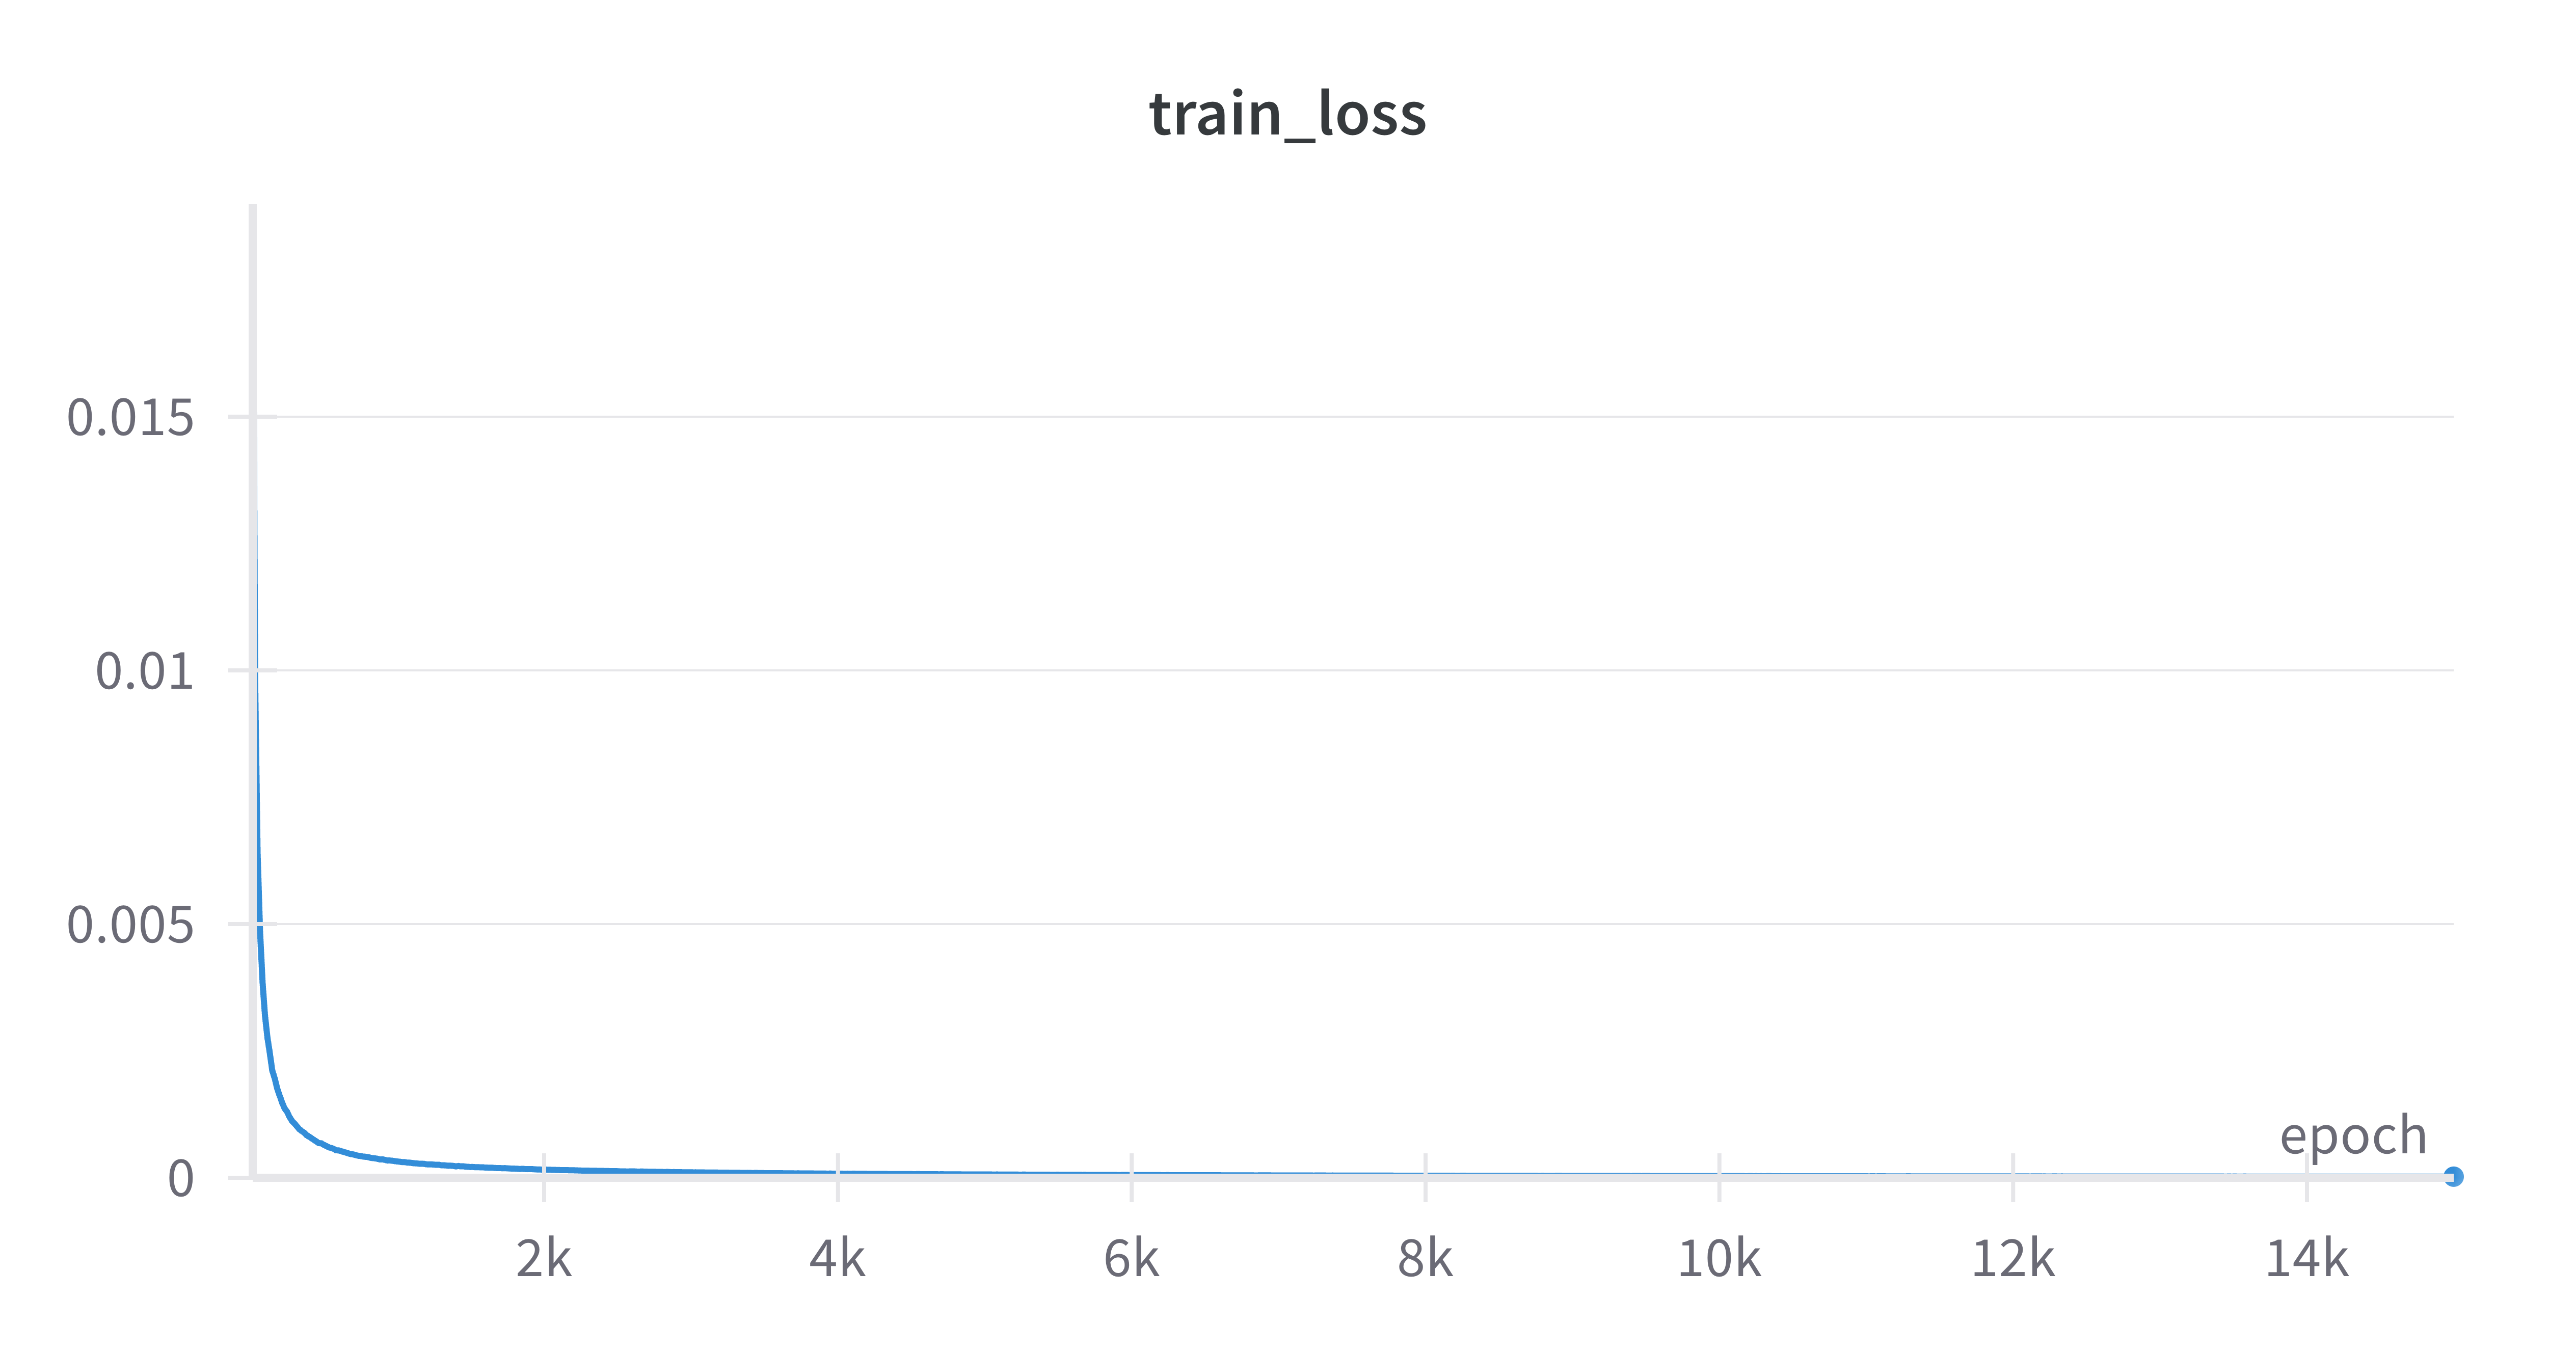
\includegraphics[width=\linewidth]{detailed_engineering/Monai Diffusion - Attempt 2/charts/train_loss.png}
\caption{}
\endminipage\hfill
\minipage{0.49\textwidth}
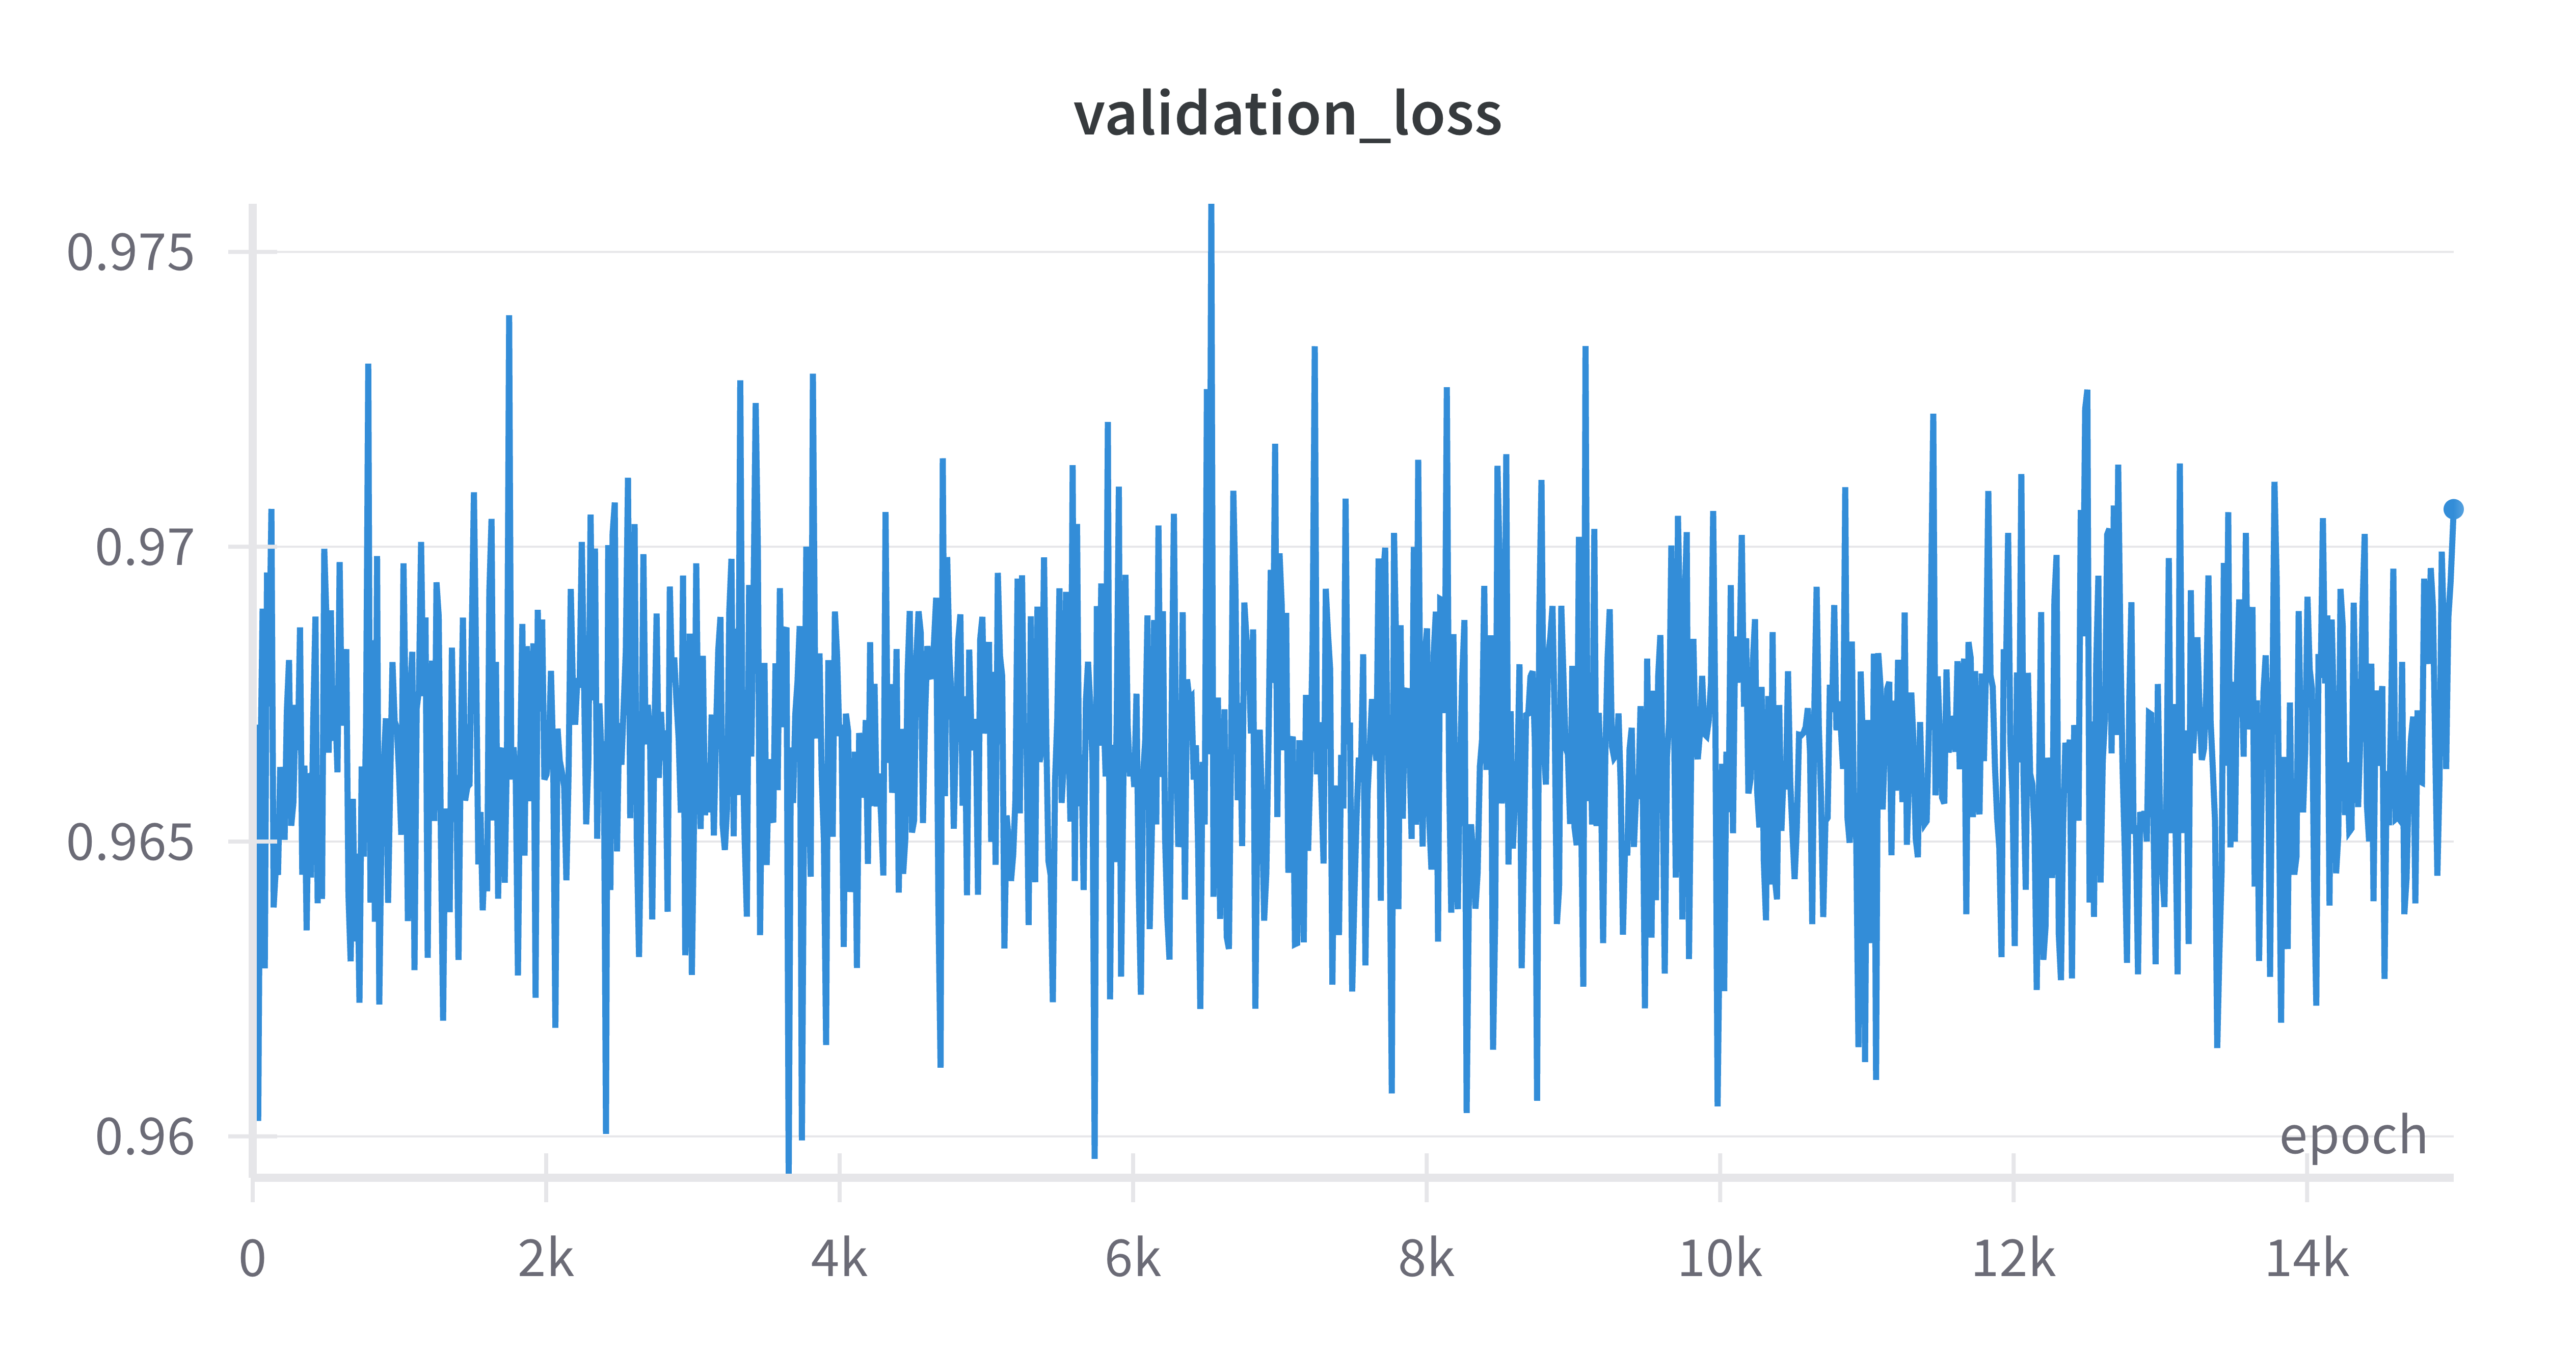
\includegraphics[width=\linewidth]{detailed_engineering/Monai Diffusion - Attempt 2/charts/validation_loss.png}
\caption{}
\label{fig:ldm_a2_val_loss}
\endminipage
\end{figure}

As is visible in the figure \ref{fig:ldm_a2_val_loss}, the validation loss did not decrease. The output of the generation was the same as in the previous attempt.





